\subsection{Time Difference of Arrival}
\label{subsec:03_tdoa}

The \ac{TDOA} estimation is the main component to identify the
whistle source location.
Theoretical background to this approach of source localization is
given in \cref{sec:02_tdoa}.
As stated there, the \ac{TDOA} of a signal measured between two microphone sensors
provides details about the direction of the source.
Having four channels attached on a NAO's head, an overdetermined system it
given where each channel pair provides \ac{TDOA} information.

The \ac{GCC-PHAT} method is a modification of the \ac{CC} method.
Due to their implementation being equal except of the weighting function,
they are discussed in \cref{subsubsec:03_cc} collectively.
\Cref{subsubsec:03_phase} presents the implementation details with it's
circumstances.
% -------------------------------------------------------------

\subsubsection{Correlation}
\label{subsubsec:03_cc}

In theory, \acf{CC} in time domain is usually illustrated by shifting
two signals about each other and recording the similarity for each shift.
Thus, a peak will arise at that shift where signals are most similar.
Imaging two equal signals, one can image a peak at the middle of the \ac{CC} function
\lstinline!R!.
The index in this case is called \lstinline!zeroIndex! and calculated with
\lstinline!int(length(R))-1!.
If one signal is alike the other but delayed by some samples, the peak will
occur at so many samples next to the \lstinline!zeroIndex!.
This delay which is directly related to the \ac{TDOA} is computed
by the \ac{CC} and \ac{GCC} in the unit of samples.
As \cref{sec:02_cc,sec:02_gcc} have shown, the \ac{GCC} is commonly performed
in frequency domain.
For unification, both \ac{CC} and \ac{GCC} are implemented in frequency domain.
% Hereinafter, \ac{CC} and \ac{GCC} will be summarized as \textit{correlation} in this section.

The samples for the \ac{CC} are defined by the start index and the frame shift
according to \cref{subsec:03_directionEstimation} and originate from the data which was
cleaned by spectral subtraction previously.
The frame size in this work is set to 256 samples typically and the samples are Hann-windowed
prior to the correlation.
By zero padding the \ac{FFT} resolution can be increased, but is refrained from for now.
For two real signals, the \ac{CC} can be realized by time-reversing one of the signals before
the \ac{FFT} and then multiplying each component.
In the event of \ac{GCC-PHAT}, each component of the multiplication is divided by the absolute
value as the weighting function \cref{eq:02_gccPhat} defines.
After this, the cross-correlated signal is transformed back into time domain and
index of the peak \lstinline!peakIndex! is found.
The delay in samples is then computed by \lstinline!peakIndex - zeroIndex!.
In conformity with the definitions in thesis, a positive delay \lstinline!d_01!
between \lstinline!x_0! (signal at channel 0) and \lstinline!x_1! (signal at channel 1)
indicates that the signal was at channel 0 first.
% -------------------------------------------------------------

\subsubsection*{Subsample Delay}
\label{subsubsec:03_subsample}

Integer delays only offers resulting direction angles with low resolution.
To avoid this, the subsample shift estimation as in \cref{sec:02_subsampleShift}
is added to the delay estimation for both \ac{CC} and \ac{GCC}.

\subsubsection{Phase Difference}
\label{subsubsec:03_phase}

% Frame size of 64 samples -> better result
% periodicity -> maximal possible frame with given distance

There are two ways to determine the angle by phase difference
between two channels.
One can either look at the phase of a fixed frequency or set the frequency
dynamically.
For both, the signal must be divided into multiple frames.
The implementation for the fixed frequency case is straight forward.
From the result of the signal start detection, the frames
are set with an appropriate frame size and then transformed into
frequency domain.
As known from \cite{Hasselbring}, the frequency of the whistle is between 2\si{\kilo\hertz}
and 4\si{\kilo\hertz}.
Thus, a suitable frequency in this range is chosen for analysis.
In the other case, the frame is chosen by doing a
frequency analysis.
For each channel frame in frequency domain after signal start,
the maximal absolute value and its belonging frequency is determined.
If this frequency is equal for all channels, these frames
are chosen.
\Cref{fig:03_maxFreq} shows that such frames exists for signals that
were transformed into frequency domain with a frame size of 256.
The frequency resolution changes with zero padding the signal prior
to the transformation.
\change[]{Finalize!}
% -------------------------------------------------------------
\begin{figure}[ht]
	\centering
		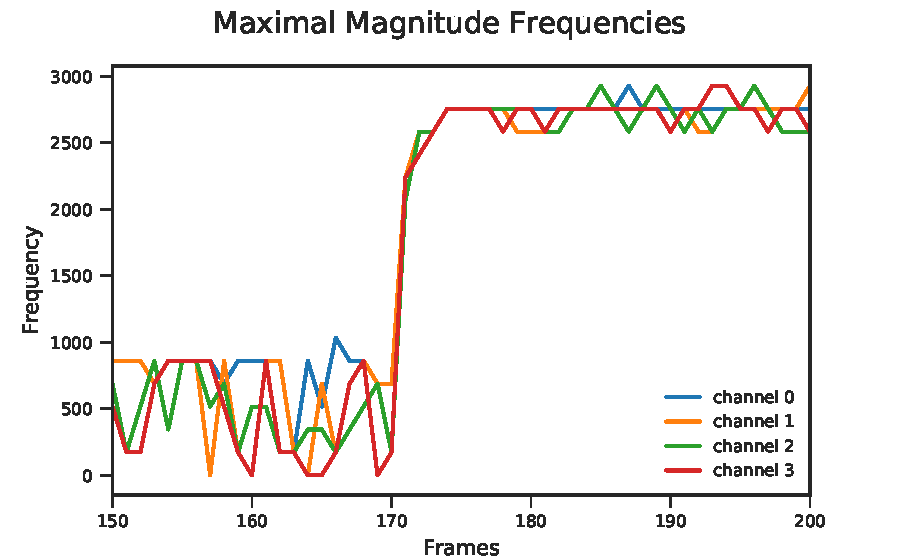
\includegraphics[]{figures/maxFreq}
	\caption{}
    \label{fig:03_maxFreq}
\end{figure}
% -------------------------------------------------------------

If the \ac{TDOA} is determined by phase difference, it must be ensured
that the maximal difference between two channels must not overflow $\pi$.
Meeting this condition, the signed difference is ascertainable.
As \cref{tab:03_maxFrequncies} presents, the distance between channel 0 and 1
is too large because its maximal frequency is not in whistle frequency range.
For this reason, the phase difference information between this pair is neglected.
% -------------------------------------------------------------
\btline{ht}{1.2}
\btab{|c|c|c|}
\hline
Channel Pairs & Absolute Distance [\si{\meter}] & Max. Frequency [\si{\hertz}]\\
\hline
0 and 1 & 0,116 & 1536,75\\
\hline
1 and 3 & 0,0533 & 3217,11\\
\hline
2 and 0 & 0,0533 & 3217,11\\
\hline
2 and 3 & 0.0618 & 2775,08\\
\hline
\etab
\et{Maximal feasible frequencies for unambiguous phase difference detection}{03_maxFrequncies}
% -------------------------------------------------------------

To facilitate the implementation, the phase difference is easily convertible into
delay samples $D_s$ with
\bal
	D_s = \frac{f_s \cdot \Delta \psi}{2 \pi \cdot f_c}.
\eal